\begin{figure}[h!]
       \centering
        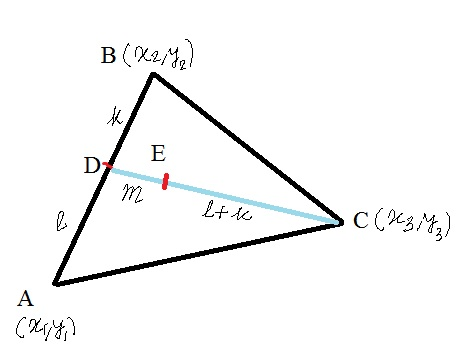
\includegraphics[width =\linewidth]{solutions/2/22/assignment1.jpg}
        \caption{Triangle ABC with vertices $\vec{A}\myvec{2\\4}$, $\vec{B}\myvec{0\\0}$, $\vec{C}\myvec{4\\0}$, and $\myvec{l\\m\\k}=\myvec{0.5\\0.5\\0.5}$ are used for python plot.The point of section $\vec{P}=\myvec{2\\0}$, $\vec{Q}=\myvec{2\\1.33}$.}\label{2/22/t1}
\end{figure}
In  Fig.\ref{2/22/t1}
\begin{align}
    \vec{B}=\myvec{x_1\\y_1},
    \vec{C}=\myvec{x_2\\y_2},
     \vec{A}=\myvec{x_3\\y_3}
\end{align}
Using section formula,
\begin{align}
    \vec{P}=\frac{l\vec{C}+k\vec{B}}{l+k}\label{2/22/yt}
\end{align}
Now,the line joining PA divided into the ratio m:k+l at point of division $\vec{Q}$ can be written by using section formula 
\begin{align}
    \vec{Q}=\frac{m\vec{A}+\brak{k+l}\vec{P}}{l+k+m}\label{2/22/t45}
\end{align}
From Eq.\eqref{2/22/yt} substitute $\vec{P}$ in Eq.\eqref{2/22/t45}
\begin{align}
    \vec{Q}&=\frac{l\vec{C}+k\vec{B}+m\vec{A}}{l+k+m} \\
    &=\frac{1}{l+k+m}\myvec{\vec{C} & \vec{B} & \vec{A}}\myvec{l\\k\\m}
\end{align}
